\section{Problem Set 5}
\subsection{Control Objectives} \label{sec:control_objectives}
\subsubsection{Operational Modes}
The ultimate goal of our formation is to demonstrate on-orbit servicing of an uncontrollable target spacecraft with a swarm of one docking satellite and one observing satellite. Specifically, the Target spacecraft (SV1) has no maneuvering capabilities as it has run out of propellant, and our formation is aiming to refuel it. As such, SV1 will act as the origin of the RTN frame and remain there throughout all of our operational modes. The Watcher spacecraft (SV2) has sensing capabilities, including optical cameras such as those in the NASA Starling mission, which will be used to inspect the Target and estimate its pose for servicing purposes. The Docker spacecraft (SV3) also has optical sensors that will aid in this inspection, but also play a crucial role in proximity and docking operations. Our formation aims to demonstrate a significant advance in on-orbit pose estimation and characterization of objects, along with improved docking operations through the use of multiple spacecraft with a variety of sensor modalities. 

In order to achieve this, the significant operational modes of our formation are as follows: 

\begin{enumerate}
\item \textbf{Initial Checkout Mode} - Initial checkout of Target spacecraft with both Watcher and Docker less than a kilometer and more than 200 meters away at closest approach to allow for vision-based sensing
\item \textbf{Approach Mode} - Docker approaches the Target while Watcher watches from the same distance. This mode runs until the Docker is approximately 10 meters away from the Target
\item \textbf{Proximity Operations Mode} - Docker completes final approach Target while Watcher watches
\item \textbf{Docked Mode} - Docker docks and services Target while Watcher watches
\item \textbf{Station Keeping Mode} - Watcher and Target stay within prescribed limits of relative eccentricity and relative inclination to remain passively safe. This mode will be applied whenever the formation is not reconfiguring. 
\end{enumerate}

\subsubsection{Operational Mode ROEs}
The absolute motion of our spacecraft is not the focus, as our formation is purely concerned with servicing a satellite. As such, all of the operational modes are defined as deputy ROEs as follows. Note that the Approach mode was split into two separate waypoints (Mode 2 and Mode 3) to better illustrate the reconfiguration. 

\begin{table}[h!]
\centering
\begin{tabular}{|c|rrrrrr|rrrrrr|}
\hline
\textbf{Mode} & \multicolumn{6}{c|}{\textbf{SV2 (m)}} & \multicolumn{6}{c|}{\textbf{SV3 (m)}} \\
\cline{2-13}
 & $d_a$ & $d_\lambda$ & $d_{e_x}$ & $d_{e_y}$ & $d_{i_x}$ & $d_{i_y}$ 
 & $d_a$ & $d_\lambda$ & $d_{e_x}$ & $d_{e_y}$ & $d_{i_x}$ & $d_{i_y}$ \\
\hline
1 & 0 & 0 & 0 & 300 & 0 & 300 & 0 & 0 & 0 & 250 & 0 & -250 \\
2 & 0 & 0 & 0 & 300 & 0 & 300 & 0 & 0 & 0 & 100 & 0 & -100 \\
3 & 0 & 0 & 0 & 300 & 0 & 300 & 0 & 0 & 0 & 10  & 0 & -10 \\
4 & 0 & 0 & 0 & 300 & 0 & 300 & 0 & 0 & 0 & 1   & 0 & -1 \\
\hline
\end{tabular}
\caption{Relative Orbital Element Modes for SV2 and SV3 (scaled by $a_c$)}
\label{tab:roe_modes}
\end{table}

These ROE values were chosen to meet the minimum separation requirements outlined above, by using the following equation:

\begin{align*}
R_{\min} &= \frac{\sqrt{2} \cdot a \cdot |\delta e \cdot \delta i|}{\text{\sqrt{(\delta e)^2 + (\delta i)^2 + |\delta e + \delta i| \cdot |\delta e - \delta i|}}
\end{align*}

Plotting this equation in 3D shows that the minimum distance is dominated by the minimum of the given $\delta e$ and $\delta i$, as shown by Figure \ref{fig:min_dist_contour}.
\begin{figure}[H]
    \centering
    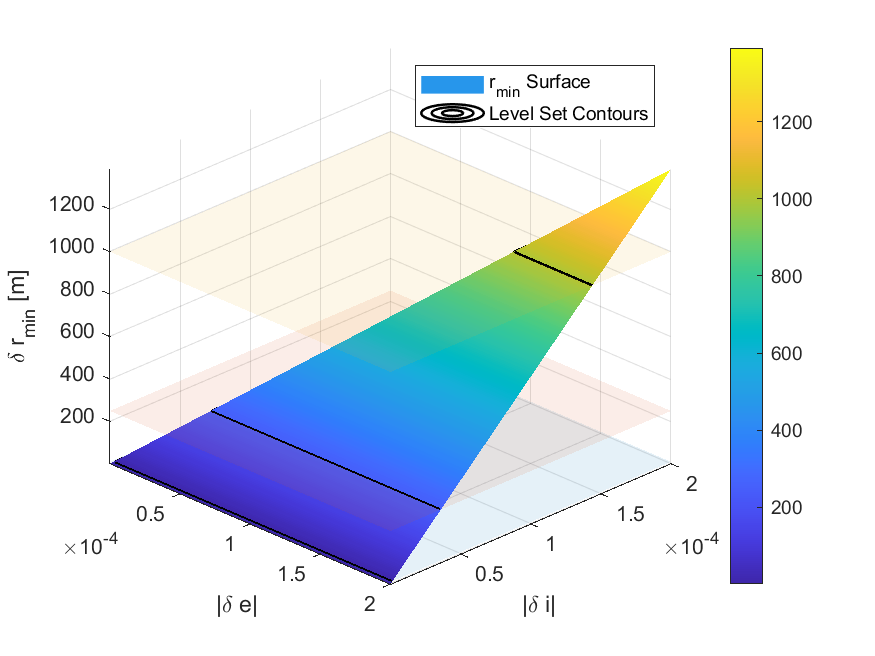
\includegraphics[width=0.75\linewidth]{sim/figures/PS5/min_dist_contour.png}
    \caption{Minimum distance contour over relative eccentricity and relative inclination}
    \label{fig:min_dist_contour}
\end{figure}
As such, $\delta e$ and $\delta i$ were chosen to be equal in magnitude for both SV2 and SV3 in order to give circular relative motion, which is helpful for maintaining the same distance throughout an orbit for the vision-based sensing on both spacecraft. Additionally, $\delta e$ and $\delta i$ were chosen to be antiparallel for SV3 (Docker) and parallel for SV2 (Watcher) to ensure that the Docker never blocks the Watcher's view of the Target by tilting the Docker's relative orbit perpendicular to the Watcher's.

\subsubsection{Formation Keeping Control Requirements}
For each station keeping mode, a keep-in region was defined for the relative eccentricity and relative inclination in order to ensure passive safety and maintain the allowable separations defined earlier. Due to the small size of the relative eccentricity and relative inclination vectors during our operational modes, a tight keep-in region of a circle with a 1-meter radius was used. 

This tight keep-in region dictates a tight relative position knowledge requirement: the Watcher's knowledge should be less than a meter and the Docker's should be less than a centimeter in order to allow for successful docking and servicing. Similarly, the velocity estimation of the Docker should be on order of mm/s.

Additionally, the actuation needed will be low-thrust, high-preicison with a low impulse bit on the order of mm/s, such as a cold gas thruster. Short, impulsive bursts will be used so to not disturb the attitude of the Docker and allow for precise control. 


\subsubsection{Reconfiguration Control Requirements}
For reconfiguration, there must always be passive safety, which is achieved through aligning the relative eccentricity and relative inclination vectors. Additionally the time to reconfigure, given in number of orbits, is prescribed for each mode below. These numbers were chosen to best illustrate the control behavior. In practice, the Approach Mode would take the longest time, especially in proximity operations where the maneuvers are small and need to be precise. 

\begin{table}[h!]
\centering
\begin{tabular}{|c|c|}
\hline
\textbf{Phase} & \textbf{Number of Orbits} \\
\hline
Mode 2 & 2 \\
Station-Keeping 2 & 3 \\
Mode 3 & 2 \\
Station-Keeping 3 & 3 \\
Mode 4 & 2 \\
\hline
\end{tabular}
\caption{Number of orbits spent in each mode and station-keeping phase}
\end{table}

\subsubsection{Choice of Actuators}
Two different types of actuators will be used. The first will be higher-thrust and lower specific impulse chemical propulsion for station keeping, phasing, and the approach. Electric propulsion is also an option here as it has higher specific impulse, but will not be used for now as impulsive delta-v's are simpler to model. The second kind of actuator used with be lower-thrust propulsion, such as cold-gas thrusters. These will be used for proximity and docking operations, as fine and accurate thrust control with small impulse bits is required. Cold gas thrusters will be used instead of hydrazine thrusters since they are less hazardous to work with. 

\subsubsection{Absolute and Relative Orbit Dynamics Models}
Two dynamics models are needed: the first will be the ground-truth and the second will actually run onboard the computationally-limited spacecraft. The absolute ground-truth will be given by numerical integration of the Fundamental Orbital Differential Equation (FODE) with J2 effects for the chief and both deputies. The relative ground-truth will be calculated by taking the differences in the absolute states and converting to the RTN and ROE representations. The onboard dynamics model cannot perform numerical integration as this would be too computationally-expensive. Instead, the absolute and onboard dynamics will be given by the analytical STM with J2 for ROE as outlined in Section \ref{sec:j2_analytical_roe}.  

Implementing the ground-truth model in open-loop shows each desired mode in the RN plane. 



\subsection{Impulsive Control Law}

\subsubsection{Control Method Considerations}

As highlighted in Section \ref{sec:control_objectives}, our system has four distinct operational modes, each with their own unique control accuracy and safety requirements. We also have control considerations for the maneuvers for transitioning between different modes.

Based on the requirements detailed in the previous section, we decided on the operational methods highlighted in Table \ref{}. Note here, that just the Docker (SV3) that performs the approach towards SV1, and so its control schemes change with time. SV2, on the other 



\definecolor{lightgray}{gray}{0.9}



\begin{table}[ht]
    \centering
    \caption{Control Methods by Mode of Operation}
    \renewcommand{\arraystretch}{1.3}

    \begin{tabularx}{\textwidth}{|>{\raggedright\arraybackslash}p{0.20\textwidth}|%
                                      >{\raggedright\arraybackslash}p{0.18\textwidth}|%
                                      >{\raggedright\arraybackslash}X|%
                                      >{\raggedright\arraybackslash}X|%
                                      >{\raggedright\arraybackslash}p{0.16\textwidth}|}
        \rowcolor{lightgray}
        \hline
        \textbf{Mode of Operation} & \textbf{Tracked State} & \textbf{In-plane Control Method} & \textbf{Out-of-plane Control Method} & \textbf{Control Window} \\
        \hline
        General Station Keeping (SV2 and SV3) & Relative orbital elements that provide passive safety (for both SV2 and SV3) & Pairs of along-track burns & Single impulse cross-track burn & Full duration of station-keeping \\
        \hline
        Approach Transfer (Mode 2)    & Desired Mode 2 final ROE (SV3 only)  & Naive least squares control solution & Naive least squares control solution & Two orbits for transfer\\
        \hline
        Proximity Maneuvers (Mode 3) & Desired Mode 3 final ROE (SV3 only)             & Radial impulse burns & Single-impulse cross-track burn & Two or \\
        \hline
        Docked Station Keeping        & N/A (Rigid Docked State)       & [Insert in-plane method] & [Insert out-of-plane method] & Continuous \\
        \hline
    \end{tabularx}
    \label{tab:mode_control_methods}
\end{table}


\begin{table}[ht]
    \centering
    \caption{Control Methods by Mode of Operation}
    \renewcommand{\arraystretch}{1.3}

    \begin{tabularx}{\textwidth}{|>{\raggedright\arraybackslash}p{0.20\textwidth}|%
                                      >{\raggedright\arraybackslash}p{0.18\textwidth}|%
                                      >{\raggedright\arraybackslash}X|%
                                      >{\raggedright\arraybackslash}X|%
                                      >{\raggedright\arraybackslash}p{0.16\textwidth}|}
        \rowcolor{lightgray}
        \hline
        \textbf{Mode of Operation} & \textbf{Tracked State} & \textbf{In-plane Control Method} & \textbf{Out-of-plane Control Method} & \textbf{Control Window} \\
        \hline
        General Station Keeping (SV2 and SV3) & Relative orbital elements that provide passive safety (for both SV2 and SV3) & Pairs of along-track burns & Single impulse cross-track burns \\
        \hline
        Approach Transfer (Mode 2)    & Desired Mode 2 final ROE (SV3 only) & Naive least squares control solution & [Insert out-of-plane method] \\
        \hline
        Proximity Maneuvers (Mode 3) & Relative Position & [Insert in-plane method] & [Insert out-of-plane method] \\
        \hline
        Docked Station Keeping        & N/A (Rigid Docked State) & [Insert in-plane method] & [Insert out-of-plane method] \\
        \hline
    \end{tabularx}
    \label{tab:mode_control_methods}
\end{table}

The control windows for the different control operations are provided in Section \ref{sec:}

\subsubsection{Control Maneuvers}
Although we had the different ideas for 



Only for mode 2:
* We will do higher-level guidance with a highly accurate state transition matrix (STMs) at a low rate so as to find intermediate waypoints
* We will go between those waypoints with lower-level control (simpler STM, calculate delta v at different points in the RTN frame).

If we only have modifications in the $\delta i_y$ and $\delta e_y$, then we won't need very complex waypoints, or maneuvers.

With just $\delta i_y \neq 0$ and $\delta i_x = 0$, 

With just $\delta e_y \neq 0$ and $\delta e_x = 0$ always, we would only have variations in the $\Delta \delta e_y$, which means that the maneuvers for this change will always happen at $u = \pm 90^\circ$, so at the maximum/minimum latitude points. Just FYI noting this down.
     Doing a tangential burn would change our delta lambda I believe, so I think there is a way to keep this within a dead-band.
     Will i 





\subsubsection{Justificiation and Implementation of Control}

\subsubsection{Results and Analysis of Control Performance}
